\section{Proofs}
\subsection{Proofs in \Cref{sec:gf}}
\begin{proof}[Proof of \Cref{prop:mmd-energy-smoothness}]
Recall that
\begin{align*}
E(\bm{X},\bm{w})
=
\frac{1}{2}\sum_{i,j=1}^N w^{(i)}w^{(j)} k(x^{(i)},x^{(j)})
-
\sum_{i=1}^N w^{(i)} m_\pi(x^{(i)})
+
\mathrm{const}.
\end{align*}
For any $\bm{u}=(u^{(1)},\ldots,u^{(N)})\in(\R^d)^N$, direct differentiation gives
\begin{align*}
\nabla_{\bm{X}}^2E(\bm{X},\bm{w})[\bm{u},\bm{u}]
={}&
\sum_{i,j=1}^N
w^{(i)}w^{(j)}
(u^{(i)})^\top\nabla_{11}^2 k(x^{(i)},x^{(j)})u^{(i)}
\\
&+
\sum_{i,j=1}^N
w^{(i)}w^{(j)}
(u^{(i)})^\top\nabla_{12}^2 k(x^{(i)},x^{(j)})u^{(j)}
-
\sum_{i=1}^N
w^{(i)}
(u^{(i)})^\top\nabla^2m_\pi(x^{(i)})u^{(i)}.
\end{align*}
Since $m_\pi(x)=\int k(x,y)\,\mathrm{d}\pi(y)$ and $\pi$ is a probability measure, we have
\begin{align*}
\|\nabla^2m_\pi(x)\|_{\mathrm{op}}
=
\left\|
\int\nabla_{11}^2 k(x,y)\,\mathrm{d}\pi(y)
\right\|_{\mathrm{op}}
\leq
\sup_{x,y\in\R^d}
\|\nabla_{11}^2 k(x,y)\|_{\mathrm{op}} = C_1.
\end{align*}
Using $\sum_{j=1}^Nw^{(j)}=1$, it follows that
\begin{align*}
\left|
\sum_{i,j=1}^N w^{(i)} w^{(j)} (u^{(i)})^\top\nabla_{11}^2 k(x^{(i)},x^{(j)})u^{(i)} - \sum_{i=1}^N w^{(i)} (u^{(i)})^\top\nabla^2m_\pi(x^{(i)})u^{(i)}
\right| \leq 2 C_1
\sum_{i=1}^Nw^{(i)}\|u^{(i)}\|^2.
\end{align*}
For the mixed term,
\begin{align*}
\left|
\sum_{i,j=1}^N
w^{(i)}w^{(j)}
(u^{(i)})^\top\nabla_{12}^2 k(x^{(i)},x^{(j)})u^{(j)}
\right|
&\leq
\sup_{x,y\in\R^d}
\|\nabla_{12}^2 k(x,y)\|_{\mathrm{op}}
\left(\sum_{i=1}^Nw^{(i)}\|u^{(i)}\|\right)^2 \\
&= C_2 \left(\sum_{i=1}^Nw^{(i)}\|u^{(i)}\|\right)^2 .
\end{align*}
By Cauchy--Schwarz and $\sum_{i=1}^Nw^{(i)}=1$, we have
$\left(\sum_{i=1}^N w^{(i)}\|u^{(i)}\|\right)^2
\leq \sum_{i=1}^Nw^{(i)}\|u^{(i)}\|^2$. Therefore,
\begin{align*}
\left|
\nabla_{\bm{X}}^2 E(\bm{X},\bm{w})[\bm{u},\bm{u}]
\right| \leq \left( 2C_1 + C_2\right) \sum_{i=1}^N w^{(i)}\|u^{(i)}\|^2 = \left( 2C_1 + C_2\right) \|\bm{u}\|_{\bm{w}}^2.
\end{align*}
The last step holds by the definition of $\bm{w}$-weighted Euclidean geometry in \Cref{defi:weighted_euc}. 
This proves smoothness under the weighted Euclidean geometry.

For the standard Euclidean geometry, since $\sum_{i=1}^Nw^{(i)}\|u^{(i)}\|^2
\leq
\left(\max_{1\leq i\leq N}w^{(i)}\right)
\sum_{i=1}^N\|u^{(i)}\|^2
=
\left(\max_{1\leq i\leq N}w^{(i)}\right)
\|\bm{u}\|_2^2$. 
This proves the first claim.

For fixed $\bm{X}$, the weight gradient is $\nabla_{\bm{w}}\calE(\bm{X},\bm{w})=K(\bm{X},\bm{X})\bm{w}-m_\pi(\bm{X})$. Hence, for any $\bm{w},\bm{v}\in\R^N$, we have $\|\nabla_{\bm{w}}\calE(\bm{X},\bm{w})-\nabla_{\bm{w}}\calE(\bm{X},\bm{v})\|_2\leq\lambda_{\max}(K(\bm{X},\bm{X}))\|\bm{w}-\bm{v}\|_2$. Under the $K(\bm{X},\bm{X})$-weighted Euclidean geometry, the corresponding gradient is $\grad_K\calE(\bm{X},\bm{w})=\bm{w}-K(\bm{X},\bm{X})^{-1}m_\pi(\bm{X})$, and therefore $\|\grad_K\calE(\bm{X},\bm{w})-\grad_K\calE(\bm{X},\bm{v})\|_K=\|\bm{w}-\bm{v}\|_K$. This proves the second claim.
\end{proof}

\begin{proof}[Proof of \Cref{prop:geometry-step-sizes}]
For an $L$-smooth function $f$ under a fixed weighted Euclidean geometry, the descent lemma applied to $z^+=z-\gamma\grad_G f(z)$ gives
\begin{align*}
f(z^+)\leq f(z)-\gamma\left(1-\frac{L\gamma}{2}\right)\|\grad_G f(z)\|_G^2.
\end{align*}
Thus, the corresponding block objective is non-increasing whenever $\gamma\leq2/L$.

For E-PD, the location substep is standard Euclidean gradient descent with effective step size $\tau_X$. By \Cref{prop:mmd-energy-smoothness}, its smoothness constant is $\max_i w_t^{(i)}(2C_1+C_2)$. With $\bm{X}_{t+1}$ fixed, the weight substep is standard Euclidean gradient descent with effective step size $\tau_w$ and smoothness constant $\lambda_{\max}(K_{t+1})$. The stated bounds therefore imply
\begin{align*}
\calE(\bm{X}_{t+1},\bm{w}_{t+1})\leq\calE(\bm{X}_{t+1},\bm{w}_t)\leq\calE(\bm{X}_t,\bm{w}_t).
\end{align*}

For WFR-PD, the location substep is gradient descent under the $\operatorname{Diag}(\bm{w}_t)$-weighted Euclidean geometry with step size $\tau_X$ and smoothness constant $2C_1+C_2$. Its weight substep is standard Euclidean gradient descent with step size $\tau_w$ and smoothness constant $\lambda_{\max}(K_{t+1})$. The same descent argument gives the claimed monotonicity.

The WIFT-PD location substep is identical to that of WFR-PD and is therefore non-increasing under the stated location condition. For the implicit weight substep, its defining minimization problem and the admissible choice $\bm{w}=\bm{w}_t$ give
\begin{align*}
\calE(\bm{X}_{t+1},\bm{w}_{t+1})
+\frac{1}{2\tau_w}\|\bm{w}_{t+1}-\bm{w}_t\|_{K_{t+1}}^2
\leq\calE(\bm{X}_{t+1},\bm{w}_t).
\end{align*}
The squared norm is nonnegative for every $\tau_w>0$, so the weight substep is non-increasing without an upper bound on $\tau_w$. Combining the two substeps concludes the proof.
\end{proof}

\subsection{Proofs in \Cref{sec:pd}} 
\begin{prop}[Monotone decrease of WIFT-PD]
\label{prop:wift-monotone-descent}
Let the iterates $\mu_{N,t}=\sum_{i=1}^N w_t^{(i)}\delta_{x_t^{(i)}}$, with $\bm{X}_t=(x_t^{(1)},\ldots,x_t^{(N)})$ and $\bm{w}_t=(w_t^{(1)},\ldots,w_t^{(N)})$, be generated by WIFT-PD with step sizes $\tau_X,\tau_w>0$. Suppose that the assumptions of \Cref{prop:mmd-energy-smoothness} hold with $\bm{w}=\bm{w}_t$ and $\bm{X}=\bm{X}_{t+1}$ at every iteration, and that $\tau_X\leq 2(2C_1+C_2)^{-1}$. Then, for every $t\geq0$,
\begin{align*}
\calE(\bm{X}_{t+1},\bm{w}_{t+1})
&\leq \calE(\bm{X}_{t+1},\bm{w}_t)
\leq \calE(\bm{X}_t,\bm{w}_t),
\end{align*}
and hence $\operatorname{MMD}(\mu_{N,t+1},\pi)\leq\operatorname{MMD}(\mu_{N,t},\pi)$.
\end{prop}

\begin{proof}[Proof of \Cref{prop:wift-monotone-descent}]
For fixed $\bm{X}$ and $\bm{w}$, let
$g^{(i)}(\bm{X},\bm{w})=\sum_{j=1}^N w^{(j)}\nabla_2 k(x^{(j)},x^{(i)})-\nabla m_\pi(x^{(i)})$.
Define the squared MMD energy by
\begin{align}\label{eq:defi_mmd}
\calE(\bm{X},\bm{w})
=\frac12\operatorname{MMD}^2\left(\sum_{i=1}^N w^{(i)}\delta_{x^{(i)}},\pi\right),
\end{align}
Differentiating the squared MMD energy with respect to $x^{(i)}$ and using symmetry of the kernel gives
$\nabla_{x^{(i)}}\calE(\bm{X},\bm{w})=w^{(i)} g^{(i)}(\bm{X},\bm{w})$.
Hence, the position update of \eqref{eq:wift-pd} can be written as $x_{t+1}^{(i)}=x_t^{(i)}-\frac{\tau_X}{w_t^{(i)}} \nabla_{x^{(i)}}\calE(\bm{X}_t,\bm{w}_t)$. 
By the $(2 C_1 + C_2)$-smoothness of $\calE(\cdot,\bm{w}_t)$ with respect to the $\operatorname{Diag}(\bm{w}_t)$-weighted Euclidean geometry established in \Cref{prop:mmd-energy-smoothness}, the descent lemma gives
\begin{align}
\calE(\bm{X}_{t+1},\bm{w}_t)
&\leq \calE(\bm{X}_t,\bm{w}_t)
-\tau_X\left(1-\frac{(2C_1+C_2)\tau_X}{2}\right)
\left\|\grad_{\operatorname{Diag}(\bm{w}_t)}
\calE(\bm{X}_t,\bm{w}_t)\right\|_{\operatorname{Diag}(\bm{w}_t)}^2
\nonumber \\
&= \calE(\bm{X}_t,\bm{w}_t) - \tau_X \left(1 - \frac{(2 C_1 + C_2)\tau_X}{2} \right) \sum_{i=1}^N
 w_t^{(i)} \left\| g^{(i)}(\bm{X}_t,\bm{w}_t)
\right\|^2.
\label{eq:wasserstein-descent}
\end{align}
Since $\tau_X\leq2(2C_1+C_2)^{-1}$, this proves that $\calE(\bm{X}_{t+1},\bm{w}_t)\leq\calE(\bm{X}_t,\bm{w}_t)$ so the location update in \eqref{eq:wift-pd} decreases the MMD value. 

We next consider the weight update. For fixed $\bm{X}$, the dependence of the MMD energy on $\bm{w}$ is quadratic:
$\calE(\bm{X},\bm{w})=\frac12 \bm{w}^\top K(\bm{X})\bm{w}-m_\pi(\bm{X})^\top \bm{w}+$const. Since $K(\bm{X})$ is positive definite, the unique minimizer is
$\bm{w}_{\mathrm{KQ}}(\bm{X})=K(\bm{X})^{-1}m_\pi(\bm{X})$.
Completing the square gives
\begin{align}
\calE(\bm{X},\bm{w})
=
\calE\left(\bm{X},\bm{w}_{\mathrm{KQ}}(\bm{X})\right)
+
\frac12 \left( \bm{w}-\bm{w}_{\mathrm{KQ}}(\bm{X}) \right)^\top K(\bm{X}) \left( \bm{w}-\bm{w}_{\mathrm{KQ}}(\bm{X}) \right).  
\label{eq:mmd-kq-decomposition}
\end{align}
Hence for fixed particle locations $\bm{X}_{t+1}$, the KQ decomposition gives
\begin{align}
&
\calE(\bm{X}_{t+1},\bm{w}_{t+1})
-
\calE\left(
\bm{X}_{t+1},
\bm{w}_{\mathrm{KQ}}(\bm{X}_{t+1})
\right)
\nonumber\\
&\qquad=
\frac{1}{2}
\left(
\bm{w}_{t+1}
-
\bm{w}_{\mathrm{KQ}}(\bm{X}_{t+1})
\right)^\top
K_{t+1}
\left(
\bm{w}_{t+1}
-
\bm{w}_{\mathrm{KQ}}(\bm{X}_{t+1})
\right).
\label{eq:kq-energy-gap}
\end{align}
Also, by the weight update,
\begin{align}
\bm{w}_{t+1} - \bm{w}_{\mathrm{KQ}}(\bm{X}_{t+1}) = \frac{1}{1+\tau_w} \left( \bm{w}_t - \bm{w}_{\mathrm{KQ}}(\bm{X}_{t+1})
\right).
\label{eq:weight-difference-contraction}
\end{align}
Substituting Eq.~\eqref{eq:weight-difference-contraction} into
Eq.~\eqref{eq:kq-energy-gap} yields
\begin{align}
&\calE(\bm{X}_{t+1},\bm{w}_{t+1})
-
\calE \left(
\bm{X}_{t+1},
\bm{w}_{\mathrm{KQ}}(\bm{X}_{t+1})
\right)
\nonumber\\
&\qquad=
\frac{1}{2(1+\tau_w)^2}
\left(
\bm{w}_t -
\bm{w}_{\mathrm{KQ}}(\bm{X}_{t+1})
\right)^\top
K_{t+1}
\left(
\bm{w}_t
-
\bm{w}_{\mathrm{KQ}}(\bm{X}_{t+1})
\right)
\nonumber\\
&\qquad=
\frac{1}{(1+\tau_w)^2}
\left[ \calE(\bm{X}_{t+1},\bm{w}_t)
-
\calE\left(
\bm{X}_{t+1},
\bm{w}_{\mathrm{KQ}}(\bm{X}_{t+1})
\right)
\right].
\label{eq:kq-weight-contraction}
\end{align}
Since $(1+\tau_w)^{-2}\leq1$ and $\bm{w}_{\mathrm{KQ}}(\bm{X}_{t+1})$ minimizes
$\bm{w}\mapsto\calE(\bm{X}_{t+1}, \bm{w})$, it follows that
$\calE(\bm{X}_{t+1},\bm{w}_{t+1})
\leq
\calE(\bm{X}_{t+1},\bm{w}_t)$.
Combining the two sub-steps yields
\begin{align}
\calE(\bm{X}_{t+1},\bm{w}_{t+1})
\leq
\calE(\bm{X}_{t+1},\bm{w}_t)
\leq
\calE(\bm{X}_t,\bm{w}_t).
\label{eq:full-wift-descent}
\end{align}
Hence, $\calE(\bm{X}_t,\bm{w}_t)$ is nonincreasing, and the proof is concluded.
\end{proof}

\begin{lem}[Uniform control of the kernel quadrature residual]
\label{lem:kq-residual-control}
Suppose that the assumptions of \Cref{prop:wift-monotone-descent} hold and that the initial weights are chosen as $\bm{w}_0=\bm{w}_{\mathrm{KQ}}(\bm{X}_0)$.
Then, for every $t\geq 0$, $\operatorname{MMD}
\left(
\sum_{i=1}^N
w_{\mathrm{KQ}}^{(i)} (\bm{X}_t)
\delta_{x_t^{(i)}},
\pi
\right)
\leq
\operatorname{MMD}
\left(
\sum_{i=1}^N
w_{\mathrm{KQ}}^{(i)}(\bm{X}_0)
\delta_{x_0^{(i)}},
\pi
\right)$.
\end{lem}


\begin{proof}[Proof of \Cref{lem:kq-residual-control}]
Recall the definition that $\calE(\bm{X},\bm{w})
=\frac12\operatorname{MMD}^2\left(\sum_{i=1}^N w^{(i)}\delta_{x^{(i)}},\pi\right)$. For any fixed particle locations $\bm{X}_t$, the kernel quadrature weights
$\bm{w}_{\mathrm{KQ}}(\bm{X}_t)$ minimize the MMD energy over the weights. Hence, $\calE\left(
\bm{X}_t,
\bm{w}_{\mathrm{KQ}}(\bm{X}_t)
\right)
\leq
\calE\left(
\bm{X}_t,
\bm{w}_t
\right)$. On the other hand, by the monotonicity of the WIFT iteration established in
\Cref{prop:wift-monotone-descent}, we have $\calE\left(
\bm{X}_t,
\bm{w}_t
\right)
\leq
\calE\left(
\bm{X}_0,
\bm{w}_0
\right)$. Since $\bm{w}_0=\bm{w}_{\mathrm{KQ}}(\bm{X}_0)$, we have
$ \calE(\bm{X}_0,\bm{w}_0)
=
\calE(\bm{X}_0,\bm{w}_{\mathrm{KQ}}(\bm{X}_0)) $.
Combining the previous inequalities gives
\begin{align}
\calE\left(
\bm{X}_t,
\bm{w}_{\mathrm{KQ}}(\bm{X}_t)
\right) \leq
\calE\left(
\bm{X}_t,
\bm{w}_t
\right) \leq
\calE\left(
\bm{X}_0,
\bm{w}_0
\right) = \calE\left(
\bm{X}_0,
\bm{w}_{\mathrm{KQ}}(\bm{X}_0)
\right).
\end{align}
The proof is thus concluded. 
\end{proof}

\begin{theorem}[Convergence; verbatim of \Cref{thm:wift-convergence}] 
\label{thm:wift-convergence-copy}
Let the iterates $\mu_{N,t}=\sum_{i=1}^N w_t^{(i)}\delta_{x_t^{(i)}}$, with $\bm{X}_t=(x_t^{(1)},\ldots,x_t^{(N)})$ and $\bm{w}_t=(w_t^{(1)},\ldots,w_t^{(N)})$, be generated by WIFT-PD with step sizes $\tau_X,\tau_w>0$. The initial weights are chosen as $\bm{w}_0=\bm{w}_{\mathrm{KQ}}(\bm{X}_0)$. 
If $\tau_X\leq 2(2C_1+C_2)^{-1}$, then for every $t\geq0$, 
\begin{align*}
\calE \left(\bm{X}_t, \bm{w}_t\right) \leq \frac{1}{(1+\tau_w)^{2 t}} \calE(\bm{X}_0, \bm{w}_{\mathrm{KQ}}(\bm{X}_0))  + \sum_{s=1}^t \left( \frac{1}{(1+\tau_w)^{2(t-s)}} - \frac{1}{(1+\tau_w)^{2(t-s+1)}} \right) \calE(\bm{X}_s, \bm{w}_{\mathrm{KQ}}(\bm{X}_s)). 
\end{align*}
\end{theorem}

\begin{proof}[Proof of \Cref{thm:wift-convergence-copy}]
\labeltheoremproof{proof:wift-convergence}{thm:wift-convergence}
From the exact contraction of the weight update in
Eq.~\eqref{eq:kq-weight-contraction}, together with descent of the Wasserstein position update, we have
\begin{align}
\calE(\bm{X}_{t+1},\bm{w}_{t+1}) \leq \frac{1}{(1+\tau_w)^2}
\calE(\bm{X}_t,\bm{w}_t) + \left(
1 - \frac{1}{(1+\tau_w)^2}
\right)
\calE \left(
\bm{X}_{t+1},
\bm{w}_{\mathrm{KQ}}(\bm{X}_{t+1}) \right).
\label{eq:wift-one-step-convergence}
\end{align}
Applying the same iteration above recursively, then we obtain, 
\begin{align*}
\calE \left(\bm{X}_{t+1}, \bm{w}_{t+1} \right) &\leq \frac{1}{(1+\tau_w)^{2 t}} \calE(\bm{X}_0, \bm{w}_0) +\left(1-\frac{1}{(1+\tau_w)^2}\right) \sum_{s=1}^t \frac{\calE(\bm{X}_s, \bm{w}_{\mathrm{KQ}}(\bm{X}_s))}{(1+\tau_w)^{2(t-s)}} . \\
&= \frac{1}{(1+\tau_w)^{2 t}} \calE(\bm{X}_0, \bm{w}_{\mathrm{KQ}}(\bm{X}_0)) + \sum_{s=1}^t \left( \frac{1}{(1+\tau_w)^{2(t-s)}} - \frac{1}{(1+\tau_w)^{2(t-s+1)}} \right) \calE(\bm{X}_s, \bm{w}_{\mathrm{KQ}}(\bm{X}_s)). 
\end{align*} 
The proof is concluded. 
\end{proof}

\section{Close- and Far-Initialization Experiments}
\label{app:distant-initialization}

We compare two Gaussian initialization settings in two dimensions: close initialization from $\mathcal{N}((1,1),I_2)$ and far initialization from $\mathcal{N}((9,9),I_2)$. The target is $\pi=\mathcal{N}(\bm{0},I_2)$, and every run uses $N=20$ particles, seed $42$, RBF length scale $1$, and $1000$ iterations. All methods use the same seed-controlled initial cloud in each setting, and the far cloud is the close cloud translated by $(8,8)$. Euc-PD, WFR, and WIFT use the linear-plus-RBF kernel with unit linear coefficient, whereas the upstream MSIP implementation uses the RBF kernel. We use $\alpha=1$ and $\beta=0.5$ and retain the unsmoothed trajectories. Figure~\ref{fig:all_mmd} reports the sweep over $\tau\in\{0.01,0.1,1\}$. The MSIP curve for $\tau=1$ is omitted because the upstream update encounters a singular Gram matrix in both settings.

Figure~\ref{fig:appendix-particle-trajectories} adapts the trajectory visualization of \citet[Figures~4--5]{gladin2024interaction} to these two-dimensional experiments. Both axes are spatial coordinates, the blue contours represent the target density, and iteration progresses along each dotted path. Each panel shows all $20$ particles: orange crosses mark step $0$, and green circles mark step $1000$. To keep the paths readable, we use $\tau=0.01$ for Euc-PD and MSIP, $\tau=0.1$ for WFR, and $\tau=1$ for WIFT. Each row uses a common spatial window spanning the target and the corresponding Gaussian initial cloud; path segments outside that window are clipped.

\begin{figure}[p]
    \centering
    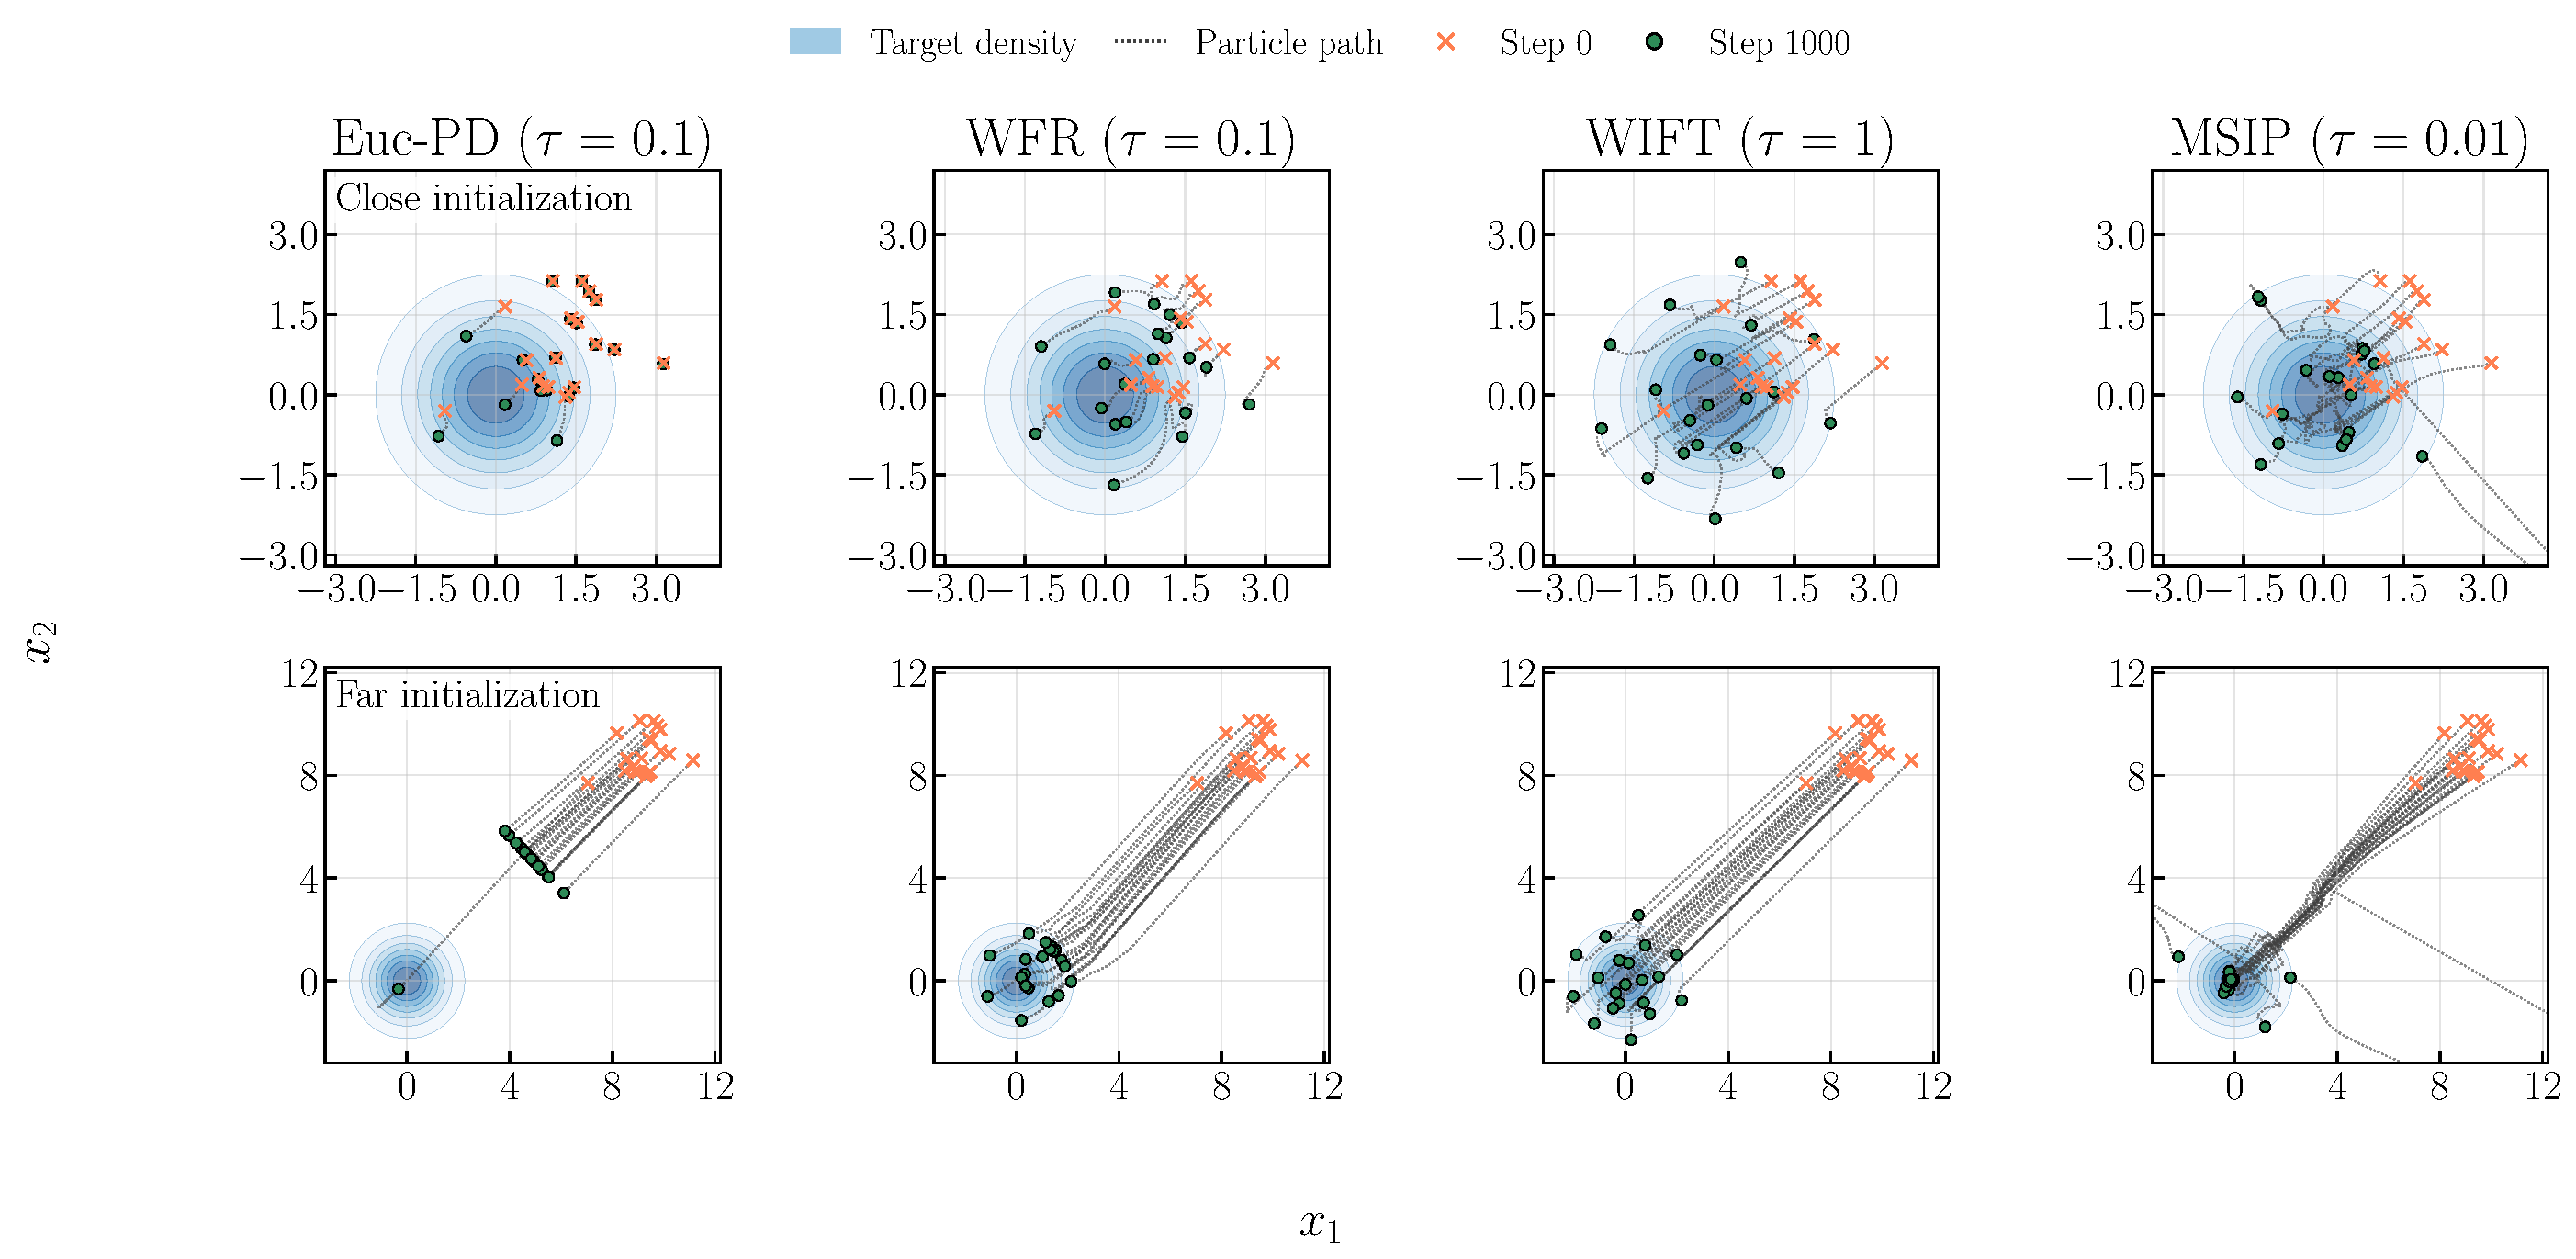
\includegraphics[width=1.0\linewidth]{figures/appendix_particle_trajectories.pdf}
    \caption{\textbf{Particle trajectories under close and far initialization.} Paths of all $20$ particles from step $0$ to step $1000$ for initial distributions $\mathcal{N}((1,1),I_2)$ and $\mathcal{N}((9,9),I_2)$, respectively.}
    \label{fig:appendix-particle-trajectories}
\end{figure}
